% Figure 1 — ML Training Pipeline
% Rich NN-architecture detail: matrix grids, embedding columns, explicit
% SAGE message passing, GRU cell internals, multi-scale TCN windows,
% gated fusion mechanism, 4-term mixture utility decomposition.
% Output: trained Theta card (5 parameter types) — bridges to Figure 2.
%
% Compile:  pdflatex figure1_ml_pipeline.tex

\documentclass[border=10pt]{standalone}

\usepackage[T1]{fontenc}
\usepackage{lmodern}
\usepackage{amsmath, amssymb}
\usepackage{tikz}
\usepackage{xcolor}
\usepackage{graphicx}

\usetikzlibrary{
  positioning, arrows.meta, shapes.geometric, calc, fit, backgrounds,
  matrix, decorations.pathmorphing, patterns,
}

% ─── Wang-inspired pastel palette + ML category accents ─────────────────────
\definecolor{stageABg}    {HTML}{E0EBF5}
\definecolor{stageABanner}{HTML}{3B6FB6}
\definecolor{stageBBg}    {HTML}{FAE5DD}
\definecolor{stageBBanner}{HTML}{C44E52}
\definecolor{cFlow}       {HTML}{E07A5F}
\definecolor{cBack}       {HTML}{8B5CF6}
\definecolor{cText}       {HTML}{1F2937}
\definecolor{cMuted}      {HTML}{6B7280}
\definecolor{cBorder}     {HTML}{CBD5E1}
\definecolor{cIO}         {HTML}{0F766E}

% Tensor cell category colours
\definecolor{cPOI}      {HTML}{93C5FD}
\definecolor{cSector}   {HTML}{86EFAC}
\definecolor{cEmp}      {HTML}{FDBA74}
\definecolor{cPop}      {HTML}{FDE68A}
\definecolor{cIMD}      {HTML}{FCA5A5}
\definecolor{cTube}     {HTML}{C4B5FD}
% Mixture utility 4-term colours (highlighted in choice head)
\definecolor{cTermV}    {HTML}{8172B2}
\definecolor{cTermBeta} {HTML}{C44E52}
\definecolor{cTermGamma}{HTML}{F59E0B}
\definecolor{cTermDelta}{HTML}{0E7490}

% Parameter category colours (for Trained Θ card)
\definecolor{cParEnc}   {HTML}{475569}
\definecolor{cParBeta}  {HTML}{C44E52}
\definecolor{cParGamma} {HTML}{F59E0B}
\definecolor{cParDelta} {HTML}{0E7490}
\definecolor{cParKappa} {HTML}{8172B2}

\begin{document}

\begin{tikzpicture}[
  font=\sffamily\small,
  thick,
  >={Stealth[length=4.5pt, width=4pt]},
  every node/.style={align=center, text=cText},
  %
  stageframe/.style={
    draw=none, fill=#1, rounded corners=6pt,
    inner xsep=10pt, inner ysep=12pt,
  },
  stagebanner/.style={
    fill=#1, text=white, font=\sffamily\bfseries\small,
    rounded corners=4pt, inner sep=6pt,
  },
  modA/.style={
    draw=stageABanner, fill=white, line width=0.7pt,
    rounded corners=3pt, inner sep=5pt,
    font=\sffamily\footnotesize,
  },
  modB/.style={
    draw=stageBBanner, fill=white, line width=0.7pt,
    rounded corners=3pt, inner sep=5pt,
    font=\sffamily\footnotesize,
  },
  iolabel/.style={font=\sffamily\scriptsize, text=cIO},
  arrFwd/.style={->, line width=1.4pt, draw=cFlow},
  arrInner/.style={->, line width=0.8pt, draw=cText!70},
  arrBack/.style={->, line width=1.0pt, draw=cBack, dashed},
  arrlbl/.style={font=\sffamily\scriptsize\itshape, text=cMuted, fill=white,
                 inner sep=1pt, midway},
  modtitle/.style={
    font=\sffamily\bfseries\footnotesize, text=#1,
  },
  cellgrid/.style={draw=cMuted!50, fill=#1, line width=0.3pt, rectangle},
]

% ════════════════════════════════════════════════════════════════════════
%  STAGE A — INPUTS (left column with explicit tensor visualisations)
% ════════════════════════════════════════════════════════════════════════

\begin{scope}[local bounding box=stageA]

  % ─── INPUT 1: X^static — N × 22 matrix with category-coloured cells (INLINE) ───
  \node[modA, anchor=north west] (xstatic) at (0, 0)
    {\begin{minipage}{60mm}
      \centering\textbf{\textcolor{stageABanner}{Input 1\,/\,3 · Static features}}\\
      \scriptsize $X^{\text{static}}\!\in\!\mathbb{R}^{N\!\times\!22}$\,(time-invariant)\\[3pt]
      \begin{tikzpicture}[scale=0.78, baseline=0]
        % column labels
        \node[font=\sffamily\tiny, text=cText] at (1.5*2.5mm, 2mm) {POI};
        \node[font=\sffamily\tiny, text=cText] at (7.5*2.5mm, 2mm) {sectors};
        \node[font=\sffamily\tiny, text=cText] at (12.5*2.5mm, 2mm) {emp};
        \node[font=\sffamily\tiny, text=cText] at (14.5*2.5mm, 2mm) {pop};
        \node[font=\sffamily\tiny, text=cText] at (16*2.5mm, 2mm) {IMD};
        \node[font=\sffamily\tiny, text=cText] at (19*2.5mm, 2mm) {tube};
        \foreach \r in {0,...,4} {
          \foreach \c in {0,1,2,3}
            \node[cellgrid=cPOI, minimum size=2.5mm] at (\c*2.5mm, -\r*2.5mm) {};
          \foreach \c [evaluate=\c as \cc using int(\c+4)] in {0,...,7}
            \node[cellgrid=cSector, minimum size=2.5mm] at (\cc*2.5mm, -\r*2.5mm) {};
          \foreach \c [evaluate=\c as \cc using int(\c+12)] in {0,1}
            \node[cellgrid=cEmp, minimum size=2.5mm] at (\cc*2.5mm, -\r*2.5mm) {};
          \foreach \c [evaluate=\c as \cc using int(\c+14)] in {0,1}
            \node[cellgrid=cPop, minimum size=2.5mm] at (\cc*2.5mm, -\r*2.5mm) {};
          \node[cellgrid=cIMD, minimum size=2.5mm] at (16*2.5mm, -\r*2.5mm) {};
          \foreach \c [evaluate=\c as \cc using int(\c+17)] in {0,...,4}
            \node[cellgrid=cTube, minimum size=2.5mm] at (\cc*2.5mm, -\r*2.5mm) {};
        }
        \node[font=\sffamily\tiny, text=cMuted] at (10.5*2.5mm, -6.0*2.5mm) {$\vdots\;1725$ rows};
      \end{tikzpicture}
    \end{minipage}};

  % ─── INPUT 2: X^dyn — 3D cube perspective (INLINE) ───
  \node[modA, below=4mm of xstatic.south, anchor=north west] (xdyn)
    {\begin{minipage}{60mm}
      \centering\textbf{\textcolor{stageABanner}{Input 2\,/\,3 · Dynamic features}}\\
      \scriptsize $X^{\text{dyn}}\!\in\!\mathbb{R}^{T\!\times\!N\!\times\!5}$\\[3pt]
      \begin{tikzpicture}[baseline=0]
        \foreach \r in {0,...,3} {
          \foreach \c in {0,...,4} {
            \node[cellgrid=stageABanner, minimum size=2.0mm,
                   opacity={0.30+0.15*\r}]
                  at (\c*2.0mm, -\r*2.0mm) {};
          }
        }
        \draw[fill=stageABanner!30, opacity=0.6, line width=0.3pt]
          (0, 0.8mm) -- (5*2.0mm, 0.8mm) -- (5*2.0mm + 6mm, 4mm) -- (6mm, 4mm) -- cycle;
        \draw[fill=stageABanner!20, opacity=0.6, line width=0.3pt]
          (5*2.0mm, 0.8mm) -- (5*2.0mm + 6mm, 4mm)
            -- (5*2.0mm + 6mm, 4mm - 4*2.0mm) -- (5*2.0mm, -3*2.0mm) -- cycle;
        \node[font=\sffamily\tiny, text=cMuted] at (-3mm, -3mm) {$N$};
        \node[font=\sffamily\tiny, text=cMuted] at (5mm, 5mm) {$T{=}24$};
        \node[font=\sffamily\tiny, text=cMuted] at (5*2.0mm + 8mm, -2mm) {$F{=}5$};
        \node[font=\sffamily\tiny, text=cText, anchor=west]
          at (5*2.0mm + 12mm, -1mm) {\textsf{cong z, inflow z,}};
        \node[font=\sffamily\tiny, text=cText, anchor=west]
          at (5*2.0mm + 12mm, -4mm) {\textsf{queue, $\sin h$, $\cos h$}};
      \end{tikzpicture}
    \end{minipage}};

  % ─── INPUT 3: graph + costs (INLINE) ───
  \node[modA, below=4mm of xdyn.south, anchor=north west] (xgraph)
    {\begin{minipage}{60mm}
      \centering\textbf{\textcolor{stageABanner}{Input 3\,/\,3 · Graph + costs}}\\
      \scriptsize $\mathcal{G}\!=\!(V,E)$, $t_{ij}^{(m)}, \log d_{ij}, \pi_m, \pi_k$\\[3pt]
      \begin{tikzpicture}[baseline=0]
        % London grid sample graph (left)
        \begin{scope}[shift={(0,0)}]
          \foreach \pos/\name in
            {(0,0)/n1, (5mm,2mm)/n2, (10mm,0)/n3, (5mm,-3mm)/n4, (0,-5mm)/n5,
             (10mm,-5mm)/n6, (15mm,-2mm)/n7}
             \node[circle, fill=stageABanner, minimum size=1.5mm, inner sep=0pt] (\name) at \pos {};
          \draw[stageABanner, line width=0.4pt] (n1) -- (n2) (n2) -- (n3) (n1) -- (n4)
                (n3) -- (n4) (n4) -- (n5) (n4) -- (n6) (n3) -- (n7) (n6) -- (n7);
          \node[font=\sffamily\tiny, text=cMuted] at (8mm, -8mm) {1\,km · 4-nb};
        \end{scope}
        % t_ij heatmap mini (centre)
        \begin{scope}[shift={(22mm, 0)}]
          \foreach \r in {0,...,4} {
            \foreach \c in {0,...,4} {
              \pgfmathsetmacro{\val}{0.2 + 0.15*(\r+\c)}
              \node[cellgrid=cTermBeta, minimum size=1.7mm, opacity=\val]
                    at (\c*1.7mm, -\r*1.7mm) {};
            }
          }
          \node[font=\sffamily\tiny, text=cMuted] at (4mm, -10mm) {$t_{ij}^{(m)}$};
        \end{scope}
        % π_m pie (right)
        \begin{scope}[shift={(40mm, -3mm)}]
          \draw[fill=cTermBeta!70, line width=0.3pt] (0,0) -- (0:2.5mm) arc (0:216:2.5mm) -- cycle;
          \draw[fill=cTermGamma!70, line width=0.3pt] (0,0) -- (216:2.5mm) arc (216:324:2.5mm) -- cycle;
          \draw[fill=cTermDelta!70, line width=0.3pt] (0,0) -- (324:2.5mm) arc (324:360:2.5mm) -- cycle;
          \node[font=\sffamily\tiny, text=cMuted] at (0, -5mm) {$\pi_m,\pi_k$};
        \end{scope}
      \end{tikzpicture}
    \end{minipage}};

\end{scope}

\begin{pgfonlayer}{background}
  \node[stageframe=stageABg, fit=(stageA)] (frameA) {};
\end{pgfonlayer}
\node[stagebanner=stageABanner, anchor=north west]
  at ($(frameA.north west)+(8pt, 0pt)$)
  {\textsc{Stage A · Inputs}\;\,\textmd{\itshape — feature tensors $+$ heterogeneity priors}};

% ════════════════════════════════════════════════════════════════════════
%  STAGE B — ENCODER (rich NN detail: SAGE / GRU / TCN / fusion)
% ════════════════════════════════════════════════════════════════════════

\begin{scope}[local bounding box=stageB, shift={(110mm, 0)}]

  % ── Static branch: explicit SAGE message passing (INLINE) ──
  \node[modA, anchor=north west] (sage) at (0, 0)
    {\begin{minipage}{68mm}\centering
      \textbf{\textcolor{stageABanner}{\textcircled{\scriptsize 1} Static branch · GraphSAGE $\times 2$}}\\
      \scriptsize\textcolor{cIO}{IN: $X^{\text{static}}, \mathcal{G}$}\;\;\textcolor{cIO}{OUT: $h_s\!\in\!\mathbb{R}^{N\!\times\!32}$}\\[4pt]
      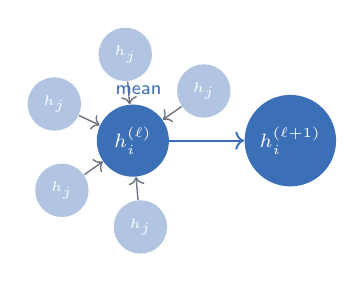
\begin{tikzpicture}[baseline=0]
        \node[circle, fill=stageABanner, minimum size=6mm, font=\sffamily\scriptsize, text=white]
          (hi) at (0, 0) {$h_i^{(\ell)}$};
        \foreach \angle/\name in {35/n1, 95/n2, 155/n3, 215/n4, 275/n5}{
          \node[circle, fill=stageABanner!40, minimum size=4mm,
                 font=\sffamily\tiny, text=white]
                (\name) at ({\angle}:11mm) {$h_j$};
          \draw[->, line width=0.5pt, draw=cMuted] (\name) -- (hi);
        }
        \node[font=\sffamily\scriptsize, text=stageABanner, anchor=south]
           at (hi.north) {\;\;mean};
        \node[circle, fill=stageABanner, minimum size=6mm, font=\sffamily\scriptsize, text=white]
          (hi1) at (20mm, 0) {$h_i^{(\ell{+}1)}$};
        \draw[->, line width=0.7pt, draw=stageABanner] (hi.east) -- (hi1.west);
      \end{tikzpicture}\\[2pt]
      \scriptsize $h_i^{(\ell+1)}=\sigma\big(W^{(\ell)}\!\cdot\!\mathrm{mean}_{j\in\mathcal{N}(i)} h_j^{(\ell)}\big)$\\
      \tiny\textcolor{cMuted}{layer 1: $W^{(1)}{:}\,22{\to}32$;\;\;layer 2: $W^{(2)}{:}\,32{\to}32$}
    \end{minipage}};

  % ── Dynamic branch: per-hour SAGE → GRU → multi-scale TCN → fuse (INLINE) ──
  \node[modA, right=8mm of sage.north east, anchor=north west] (dyn)
    {\begin{minipage}{106mm}\centering
      \textbf{\textcolor{stageABanner}{\textcircled{\scriptsize 2} Dynamic branch · per-hour SAGE $\to$ GRU $\to$ multi-scale TCN $\to$ fuse}}\\
      \scriptsize\textcolor{cIO}{IN: $X^{\text{dyn}}\!\in\!\mathbb{R}^{T\!\times\!N\!\times\!5}, \mathcal{G}$}\;\;\textcolor{cIO}{OUT: $h_d\!\in\!\mathbb{R}^{T\!\times\!N\!\times\!32}$}\\[4pt]
      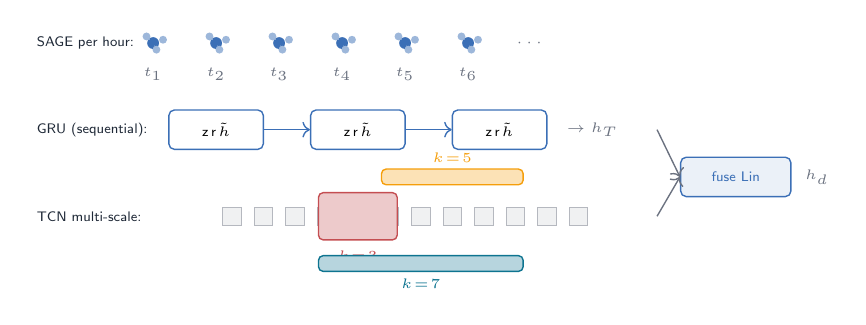
\begin{tikzpicture}[baseline=0]
        % per-hour SAGE row at top
        \node[font=\sffamily\tiny, text=cText, anchor=west] at (-2mm, 22mm) {SAGE per hour:};
        \foreach \t/\xoff in {1/14, 2/22, 3/30, 4/38, 5/46, 6/54}{
          \begin{scope}[shift={(\xoff mm, 22mm)}, scale=0.42]
            \node[circle, fill=stageABanner, minimum size=1.5mm, inner sep=0pt] (a\t) at (0,0) {};
            \node[circle, fill=stageABanner!50, minimum size=1.0mm, inner sep=0pt] (b\t) at (3mm, 1mm) {};
            \node[circle, fill=stageABanner!50, minimum size=1.0mm, inner sep=0pt] (c\t) at (-2mm, 2mm) {};
            \node[circle, fill=stageABanner!50, minimum size=1.0mm, inner sep=0pt] (d\t) at (1mm, -2mm) {};
            \draw[stageABanner!50, line width=0.2pt] (a\t)--(b\t) (a\t)--(c\t) (a\t)--(d\t);
          \end{scope}
          \node[font=\sffamily\tiny, text=cMuted] at (\xoff mm, 18mm) {$t_\t$};
        }
        \node[font=\sffamily\tiny, text=cMuted] at (62mm, 22mm) {$\cdots$};
        % GRU row middle
        \node[font=\sffamily\tiny, text=cText, anchor=west] at (-2mm, 11mm) {GRU (sequential):};
        \foreach \t/\xoff in {1/22, 2/40, 3/58}{
          \node[draw=stageABanner, rounded corners=2pt, fill=white, line width=0.5pt,
                 minimum width=12mm, minimum height=5mm,
                 font=\sffamily\tiny] (gru\t) at (\xoff mm, 11mm) {z\,r\,$\tilde h$};
        }
        \draw[->, line width=0.5pt, draw=stageABanner] (gru1.east) -- (gru2.west);
        \draw[->, line width=0.5pt, draw=stageABanner] (gru2.east) -- (gru3.west);
        \node[font=\sffamily\tiny, text=cMuted] at (70mm, 11mm) {$\!\to h_T$};
        % TCN row bottom
        \node[font=\sffamily\tiny, text=cText, anchor=west] at (-2mm, 0mm) {TCN multi-scale:};
        \foreach \i in {0,...,11}{
          \node[draw=cMuted!50, fill=cMuted!10, minimum size=2mm, line width=0.2pt]
                at (24mm + \i*4mm, 0) {};
        }
        \draw[draw=cTermBeta, fill=cTermBeta!30, line width=0.5pt, rounded corners=0.6mm]
              (24mm + 3*4mm - 1mm, -3mm) rectangle (24mm + 5*4mm + 1mm, 3mm);
        \node[font=\sffamily\tiny, text=cTermBeta] at (24mm + 4*4mm, -5mm) {$k\!=\!3$};
        \draw[draw=cTermGamma, fill=cTermGamma!30, line width=0.5pt, rounded corners=0.6mm]
              (24mm + 5*4mm - 1mm, 4mm) rectangle (24mm + 9*4mm + 1mm, 6mm);
        \node[font=\sffamily\tiny, text=cTermGamma] at (24mm + 7*4mm, 7.5mm) {$k\!=\!5$};
        \draw[draw=cTermDelta, fill=cTermDelta!30, line width=0.5pt, rounded corners=0.6mm]
              (24mm + 3*4mm - 1mm, -7mm) rectangle (24mm + 9*4mm + 1mm, -5mm);
        \node[font=\sffamily\tiny, text=cTermDelta] at (24mm + 6*4mm, -8.5mm) {$k\!=\!7$};
        % fuse linear at right
        \node[draw=stageABanner, rounded corners=2pt, fill=stageABanner!10,
               line width=0.5pt, minimum width=14mm, minimum height=5mm,
               font=\sffamily\tiny, text=stageABanner]
              (fuse) at (88mm, 5mm) {fuse Lin};
        \draw[->, line width=0.5pt, draw=cMuted] (78mm, 11mm) -- (fuse.west);
        \draw[->, line width=0.5pt, draw=cMuted] (78mm, 0mm) -- (fuse.west);
        \node[font=\sffamily\tiny, text=cMuted, anchor=west] at (fuse.east) {\;$h_d$};
      \end{tikzpicture}
    \end{minipage}};

  % ── Gated fusion (INLINE) — placed BELOW the two ──
  \node[modA, below=4mm of sage.south west, anchor=north west] (gfuse)
    {\begin{minipage}{186mm}\centering
      \textbf{\textcolor{stageABanner}{\textcircled{\scriptsize 3} Gated fusion}\;\;}
      \scriptsize\textcolor{cIO}{IN: $h_s, h_d$}\;\;\textcolor{cIO}{OUT: $V_{j,t}\!\in\!\mathbb{R}^{T\!\times\!N}$\;(then z-norm)}\\[3pt]
      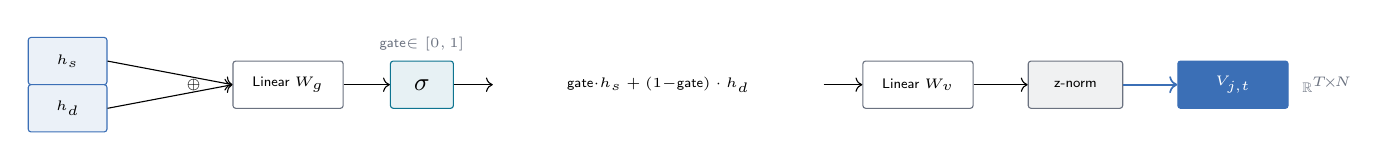
\begin{tikzpicture}[baseline=0]
        \node[draw=stageABanner, fill=stageABanner!10, rounded corners=1pt,
               minimum width=10mm, minimum height=6mm, font=\sffamily\tiny] (hs) at (0, 2mm) {$h_s$};
        \node[draw=stageABanner, fill=stageABanner!10, rounded corners=1pt,
               minimum width=10mm, minimum height=6mm, font=\sffamily\tiny] (hd) at (0, -4mm) {$h_d$};
        \node[font=\sffamily\tiny] at (16mm, -1mm) {$\oplus$};
        \node[draw=cMuted, fill=white, rounded corners=1pt,
               minimum width=14mm, minimum height=6mm, font=\sffamily\tiny] (lin) at (28mm, -1mm) {Linear $W_g$};
        \draw[->, line width=0.4pt] (hs.east) -- (lin.west);
        \draw[->, line width=0.4pt] (hd.east) -- (lin.west);
        \node[draw=cTermDelta, fill=cTermDelta!10, rounded corners=1pt,
               minimum width=8mm, minimum height=6mm, font=\sffamily\small] (sig) at (45mm, -1mm) {$\sigma$};
        \draw[->, line width=0.4pt] (lin.east) -- (sig.west);
        \node[font=\sffamily\tiny, text=cMuted, anchor=south] at (sig.north) {gate$\in[0,1]$};
        \node[font=\sffamily\tiny] at (75mm, -1mm) {gate$\cdot h_s + (1{-}$gate$)\cdot h_d$};
        \draw[->, line width=0.4pt] (sig.east) -- (54mm, -1mm);
        \node[draw=cMuted, fill=white, rounded corners=1pt,
               minimum width=14mm, minimum height=6mm, font=\sffamily\tiny] (vh) at (108mm, -1mm) {Linear $W_v$};
        \draw[->, line width=0.4pt] (96mm, -1mm) -- (vh.west);
        \node[draw=cMuted, fill=cMuted!10, rounded corners=1pt,
               minimum width=12mm, minimum height=6mm, font=\sffamily\tiny] (zn) at (128mm, -1mm) {z-norm};
        \draw[->, line width=0.4pt] (vh.east) -- (zn.west);
        \node[draw=stageABanner, fill=stageABanner, rounded corners=1pt,
               minimum width=14mm, minimum height=6mm,
               font=\sffamily\tiny, text=white] (vjt) at (148mm, -1mm) {$V_{j,t}$};
        \draw[->, line width=0.6pt, draw=stageABanner] (zn.east) -- (vjt.west);
        \node[font=\sffamily\tiny, text=cMuted, anchor=west] at (vjt.east) {\;$\mathbb{R}^{T\!\times\!N}$};
      \end{tikzpicture}
    \end{minipage}};

  % inner arrows (sage → fuse, dyn → fuse)
  \draw[arrInner] (sage.south) |- ($(gfuse.north)+(-30mm, 0)$);
  \draw[arrInner] (dyn.south) |- ($(gfuse.north)+(20mm, 0)$);

\end{scope}

\begin{pgfonlayer}{background}
  \node[stageframe=stageABg, fit=(stageB)] (frameB) {};
\end{pgfonlayer}
\node[stagebanner=stageABanner, anchor=north west]
  at ($(frameB.north west)+(8pt, 0pt)$)
  {\textsc{Stage B · Encoder}\;\,\textmd{\itshape — dual-branch ST-GNN $+$ gated fusion · 33{,}026 weights}};

% ════════════════════════════════════════════════════════════════════════
%  STAGE C — CHOICE HEAD + LOSS + TRAINED Θ OUTPUT
% ════════════════════════════════════════════════════════════════════════

\begin{scope}[local bounding box=stageC, shift={(0, -125mm)}]

  % ── ④ Choice head — 4-term mixture utility ──
  \node[modB, minimum width=120mm, minimum height=80mm,
         anchor=north west] (head) at (0, 0)
    {\begin{minipage}{116mm}\centering
      \textbf{\textcolor{stageBBanner}{\textcircled{\scriptsize 4} Choice head · mode\,$\!\times$\,tier mixture softmax}}\\
      \scriptsize\textcolor{cIO}{IN: $V_{j,t}, t_{ij}^{(m)}, \log d_{ij}, \mathrm{OccM}, \pi_m(i\!,\!j), \pi_k(i)$}\;\;
      \textcolor{cIO}{OUT: $P(j|i,t)\!\in\!\mathbb{R}^{T\!\times\!N\!\times\!N}$}
    \end{minipage}};
  % U^(m,k) = αV + βκt + γlog d + δOccM with 4 colored terms
  \begin{scope}[shift={($(head.center)+(0, 6mm)$)}]
    \node[font=\sffamily\small] at (-46mm, 0) {$U^{(m,k)}_{ij,t} =$};
    \node[draw=cTermV, fill=cTermV!15, rounded corners=2pt, line width=0.6pt,
           inner sep=2pt, font=\sffamily\footnotesize] at (-30mm, 0) {$\alpha V_{j,t}$};
    \node[font=\sffamily\small] at (-18mm, 0) {$+$};
    \node[draw=cTermBeta, fill=cTermBeta!15, rounded corners=2pt, line width=0.6pt,
           inner sep=2pt, font=\sffamily\footnotesize] at (-3mm, 0) {$\beta_{t,m} \kappa_k t_{ij}^{(m)}$};
    \node[font=\sffamily\small] at (12mm, 0) {$+$};
    \node[draw=cTermGamma, fill=cTermGamma!15, rounded corners=2pt, line width=0.6pt,
           inner sep=2pt, font=\sffamily\footnotesize] at (24mm, 0) {$\gamma \log d_{ij}$};
    \node[font=\sffamily\small] at (37mm, 0) {$+$};
    \node[draw=cTermDelta, fill=cTermDelta!15, rounded corners=2pt, line width=0.6pt,
           inner sep=2pt, font=\sffamily\footnotesize] at (50mm, 0) {$\delta_k \mathrm{OccM}_{ij}$};
    % term semantics
    \node[font=\sffamily\tiny, text=cTermV, anchor=north] at (-30mm, -3mm) {ML-learned};
    \node[font=\sffamily\tiny, text=cTermBeta, anchor=north] at (-3mm, -3mm) {time, by mode\,/\,tier};
    \node[font=\sffamily\tiny, text=cTermGamma, anchor=north] at (24mm, -3mm) {distance};
    \node[font=\sffamily\tiny, text=cTermDelta, anchor=north] at (50mm, -3mm) {occ.\ match, by tier};
  \end{scope}
  % Mixture aggregation
  \begin{scope}[shift={($(head.center)+(0, -10mm)$)}]
    \node[font=\sffamily\small] at (-30mm, 0)
      {$P(j|i,t) = \!\!\sum_{m \in \{\mathrm{car,tr,wk}\}}\!\!\!\!\pi_m(i,j)\,
        \sum_{k \in \{\mathrm{lo,mi,hi}\}}\!\!\!\!\pi_k(i)\;\,
        \mathrm{softmax}_j\,U^{(m,k)}_{ij,t}$};
  \end{scope}
  % Mixture grid: 3 modes × 3 tiers
  \begin{scope}[shift={($(head.center)+(15mm, -22mm)$)}]
    \foreach \r/\m in {0/car, 1/tr, 2/wk}{
      \foreach \c/\k in {0/lo, 1/mi, 2/hi}{
        \node[draw=cTermBeta, fill=cTermBeta!30, line width=0.4pt,
               minimum size=4mm, font=\sffamily\tiny]
              at (\c*5mm, -\r*5mm) {};
      }
    }
    % column / row labels
    \foreach \c/\k in {0/lo, 1/mi, 2/hi}
      \node[font=\sffamily\tiny, text=cMuted] at (\c*5mm, 4mm) {\k};
    \foreach \r/\m in {0/car, 1/tr, 2/wk}
      \node[font=\sffamily\tiny, text=cMuted] at (-4mm, -\r*5mm) {\m};
    \node[font=\sffamily\tiny, text=cMuted] at (5mm, -16mm) {9 softmax cells};
  \end{scope}

  % ── ⑤ Cross-entropy loss + backprop ──
  \node[modB, minimum width=80mm, minimum height=80mm, fill=stageBBanner!8,
         right=8mm of head.north east, anchor=north west] (loss)
    {\begin{minipage}{76mm}\centering
      \textbf{\textcolor{stageBBanner}{\textcircled{\scriptsize 5} Cross-entropy loss $+$ joint backprop}}\\
      \scriptsize\textcolor{cIO}{IN: $P(j|i,t), F_{ij,t}^{\mathrm{obs}}$}\;\;
      \textcolor{cIO}{OUT: trained $\Theta$}\\[3pt]
      \scriptsize $\mathcal{L} = -\!\!\sum_{i,j,t}\!\! F_{ij,t}\,\log P(j|i,t)$\\[2pt]
      \scriptsize Adam: enc lr 1e-3, head lr 1e-2; weight-decay 1e-4\\
      \scriptsize $\nabla_\Theta \mathcal{L}$ updates encoder $\Theta_{\text{enc}}$ AND choice params $(\beta,\gamma,\delta,\kappa)$ jointly\\[3pt]
      \includegraphics[width=70mm]{../figures/arch/train_curve_v2.png}\\
      \scriptsize\textit{val CPC = 0.488 (London 2019, 200 ep)}
    \end{minipage}};

  % ── ⑥ Trained Θ output card — 5 categories ──
  \node[modB, minimum width=210mm, minimum height=44mm, fill=cParEnc!4,
         below=6mm of head.south west, anchor=north west] (theta)
    {\begin{minipage}{206mm}\centering
      \textbf{\textcolor{stageBBanner}{\textcircled{\scriptsize 6} Trained $\Theta$ — output of training, frozen at deployment\;\,(bridge to Figure 2)}}
    \end{minipage}};
  \begin{scope}[shift={($(theta.south)+(-95mm, 4mm)$)}]
    % 5 colored param-type cards
    \node[draw=cParEnc, fill=cParEnc!10, rounded corners=2pt, line width=0.7pt,
           minimum width=33mm, minimum height=24mm,
           font=\sffamily\tiny, text=cParEnc, align=center] at (0, 0)
       {\textbf{$\Theta_{\text{enc}}$}\\\scriptsize\textbf{33{,}026 weights}\\\tiny deep ML, opaque\\\tiny encoder maps $X\!\to\!V_{j,t}$\\\tiny\textit{used by ALL agents}};
    \node[draw=cParBeta, fill=cParBeta!10, rounded corners=2pt, line width=0.7pt,
           minimum width=37mm, minimum height=24mm,
           font=\sffamily\tiny, text=cParBeta, align=center] at (40mm, 0)
       {\textbf{$\beta_{t,m}$ time sensitivity}\\\scriptsize\textbf{72 params (24h $\times$ 3 modes)}\\\tiny $\beta_{\text{car}}\!=\!{-}.187$\\\tiny $\beta_{\text{tr}}\!=\!{-}.105$, $\beta_{\text{wk}}\!=\!{-}.049$\\\tiny\textit{agent fetches by mode}};
    \node[draw=cParGamma, fill=cParGamma!10, rounded corners=2pt, line width=0.7pt,
           minimum width=33mm, minimum height=24mm,
           font=\sffamily\tiny, text=cParGamma, align=center] at (80mm, 0)
       {\textbf{$\gamma$ distance decay}\\\scriptsize\textbf{1 param}\\\tiny $\gamma\!=\!{-}.328$\\\tiny universal log-distance penalty\\\tiny\textit{shared by ALL agents}};
    \node[draw=cParDelta, fill=cParDelta!10, rounded corners=2pt, line width=0.7pt,
           minimum width=37mm, minimum height=24mm,
           font=\sffamily\tiny, text=cParDelta, align=center] at (120mm, 0)
       {\textbf{$\delta_k$ occ.\ matching}\\\scriptsize\textbf{2 free, $\delta_0\!=\!0$ anchor}\\\tiny $\delta_{\text{lo}}\!=\!0,\,\delta_{\text{mi}}\!=\!.20$\\\tiny $\delta_{\text{hi}}\!=\!.20$\\\tiny\textit{agent fetches by tier}};
    \node[draw=cParKappa, fill=cParKappa!10, rounded corners=2pt, line width=0.7pt,
           minimum width=37mm, minimum height=24mm,
           font=\sffamily\tiny, text=cParKappa, align=center] at (160mm, 0)
       {\textbf{$\kappa_k$ tier scaling on $\beta$}\\\scriptsize\textbf{2 free, $\kappa_0\!=\!1$ anchor}\\\tiny $\kappa_{\text{lo}}\!=\!1.00$\\\tiny $\kappa_{\text{mi}}\!=\!1.97$, $\kappa_{\text{hi}}\!=\!1.97$\\\tiny\textit{agent fetches by tier}};
  \end{scope}
  \node[font=\sffamily\scriptsize\itshape, text=cMuted, anchor=south]
      at ($(theta.south)+(0, -8mm)$)
      {\textbf{Total: 33{,}103} trainable parameters \,/\, 77 are interpretable behavioural primitives (0.23\%) — these 77 carry the paper's contribution.};

  % inner arrows
  \draw[arrInner] (head.east) -- node[arrlbl, above] {$P(j|i,t)$} (loss.west);
  \draw[arrBack]  (loss.south) .. controls ($(loss.south)+(0,-12mm)$) and ($(head.south)+(0,-12mm)$) ..
                   node[arrlbl, font=\sffamily\scriptsize, fill=white, text=cBack]
                       {$\nabla_\Theta\mathcal{L}$} (head.south);
  \draw[arrFwd] (loss.south) -- ++(0, -8mm) -| (theta.north);

\end{scope}

\begin{pgfonlayer}{background}
  \node[stageframe=stageBBg, fit=(stageC)] (frameC) {};
\end{pgfonlayer}
\node[stagebanner=stageBBanner, anchor=north west]
  at ($(frameC.north west)+(8pt, 0pt)$)
  {\textsc{Stage C · Choice head + Loss + Trained $\Theta$}\;\,\textmd{\itshape — supervised inverse learning · 77 interpretable parameters (0.23\%)}};

% ════════════════════════════════════════════════════════════════════════
%  MAIN FLOW ARROWS
% ════════════════════════════════════════════════════════════════════════

\draw[arrFwd] (frameA.east) -- node[arrlbl, above, font=\sffamily\small\bfseries]
              {tensors} (frameB.west);
\draw[arrFwd] (frameB.south) -- node[arrlbl, fill=white, font=\sffamily\small\bfseries]
              {$V_{j,t}$} (frameC.north);

% ════════════════════════════════════════════════════════════════════════
%  Footer: title and pointer to Figure 2
% ════════════════════════════════════════════════════════════════════════

\node[font=\sffamily\bfseries\large, anchor=south west, text=cText]
  at ($(frameA.north west)+(-2pt, 4mm)$)
  {Figure 1 — ML Training Pipeline\;\,
   \textmd{\itshape\large(supervised inverse learning of choice parameters from aggregate hourly OD)}};

\node[font=\sffamily\scriptsize\itshape, text=cMuted, anchor=north west,
       text width=320mm]
  at ($(frameC.south west)+(0, -6pt)$)
  {Trained $\Theta$ has \textbf{5 functional categories}:
   $\Theta_{\text{enc}}$ (deep ML, used by anyone going through encoder);
   $\beta_{t,m}$ (time sensitivity, fetched per agent's mode);
   $\gamma$ (distance, shared);
   $\delta_k$ (occ.\ match, fetched per agent's tier);
   $\kappa_k$ (tier scaling on $\beta$, fetched per agent's tier).
   These five parameter types are the bridge to Figure~2 (ABM forward simulation).};

\end{tikzpicture}

\end{document}
